\chapter{文献回顾}
本文的最终目的是处理条件生成下的图像修复问题,即在给定测量下的加工后图像,力求还原在原有数据集中极大似然意义下的原像。例如在图像\ref{original image }作为原始图像,如果去除图像中的部分像素点得到损坏图像\ref{inpainted image}。则我们的任务是已知原图像是属于FFHQ数据集,我们想要通过损坏图像\ref{inpainted image}来还愿得到最有可能属于原数据集的原像图像。    

在该图像修复问题中,涉及一下两个难点:     

1. 如何得到关于原数据集的信息,在如上例子中即为,如何获取FFHQ数据集的特征并确保最终生成图像是属于该数据集的。   

2. 如何在给定损坏图像的情形下,还原得到在极大似然估计意义下该损坏图像的原像,即需要定义何为最佳原像。    

为了应对上述两个核心问题,本章首先综述了无条件生成模型的相关文献,这一过程旨在掌握原始数据集分布的关键信息。随后,本文还总结了当前条件生成模型在图像修复领域的研究成果和贡献。
\begin{figure}[H]
  \centering
  \begin{minipage}[b]{0.45\linewidth}
    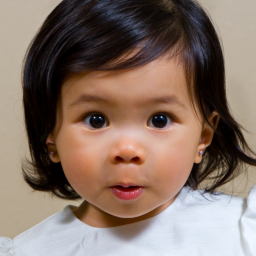
\includegraphics[width=\linewidth]{figures/intro/input.png}
    \caption{原始图像}
    \label{original image }
  \end{minipage}
  \hspace{0.5cm} % Space between images
  \begin{minipage}[b]{0.45\linewidth}
    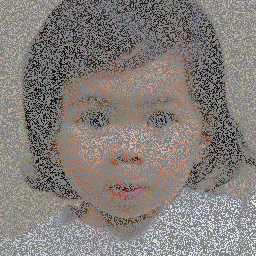
\includegraphics[width=\linewidth]{figures/intro/label.png}
    \caption{损坏图像}
    \label{inpainted image}
  \end{minipage}
\end{figure}
\section{无条件生成模型}
\subsection{变分编码器(VAE Model)}
变分编码器(Variational Auto Encoder Model)是一个有效学习未知高维数据分布的生成式模型,广泛应用于图像,音频,视频等数据用用于生成相似分布的数据, 在\cite{vae_model}中被首次提出,在例\cite{VAE_diffusion}中对于不同下游任务的特性进行了进一步的推广。在诸多Bayes模型中,通常需要构造隐式变量(Latent Variable)去用来刻画目标分布,然而通常对于隐式变量的后验分布是没有任何额外信息的,同时在许多模型下也不存在解析表达式。\par 
首先明确VAE模型的适用问题范围,VAE模型主要用来处理i.i.d型数据点样本,利用变分推断等方法获得对该连续分布数据的逼近。
在VAE模型中,引入了编码器(Encoder)用来逼近隐式变量的后验分布(基于现有样本),利用变分推断、极大似然估计等技术来训练解码器(Decoder),从而利用隐式变量生成对目标样本分布的逼近。以下为变分编码器构成的图例,在图\ref{VAE model fig}中,首先中,首先将原始数据点作为输入,利用编码器可生成隐式变量。通过在隐式变量空间中重新采样,可以重新通过解码器映射到样本空间中,生成对原样本分布的逼近。
\begin{figure}[H]
    \centering
    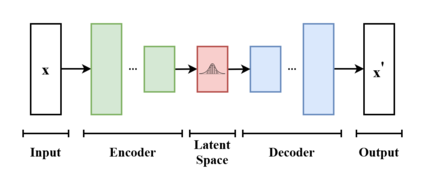
\includegraphics[scale = 0.7]{Picture/VAE.png}
    \caption{VAE 模型构成}
    \label{VAE model fig}
\end{figure}
以上为VAE模型的总体架构说明,接下来的部分将对VAE模型的数学原理进行说明。VAE模型同传统贝叶斯模型一样,同样采用极大似然估计的方法(MLE)对参数进行估计。不同点在于不直接对似然函数进行优化,采用变分推断的方法对对数似然函数的相反数下界进行极小化。该方法避免了不存在解析解的困境,易于数值计算提升优化效率。接下来定义相关符号,在VAE模型中,解码器为$p_{\theta}(x|z)$,在给定了隐式变量$z$的情况下通过以$\theta$为参数化的模型定义了一个条件概率分布。编码器$q_{\phi}(z|x)$,用来逼近真实的后验分布$p_{\theta}(z|x)$。与传统的Bayes模型不同的地方在于,编码器和解码器不直接定义从样本空间和隐式空间之间的具体映射,而是从一个空间的样本定义在另一个空间内样本的分布,再通过采样的方式获得。假设给定样本点为$\{x^1,\cdots,x^{N}\}$,在MLE的原则下,我们的目标是极大化$\mathbb{E}[\log(p_{\theta}(x))]$,
\begin{equation}
    \mathbb{E}[\log(p_{\theta}(x))] = \operatorname{KL}(q_{\phi}(z|x)||p_{\theta}(z|x)) + \mathcal{L}(x,\theta,\phi),
\end{equation}
其中$\mathcal{L}$可以写为
\begin{align}
    \mathcal{L}(x,\theta,\phi) &= \mathbb{E}_{q_{\phi}(z|x)}\left[-\log(q_{\phi}(z|x))+\log(p_{\theta}(z,x))\right]\\
    &=-\operatorname{KL}(q_{\phi}(z|x)||p_{\theta}(z))+\mathbb{E}_{q_{\phi}(z|x)}\left[p_{\theta}(x|z))\right].
\end{align}
VAE模型中一个重要假设就是需要隐式变量$z$所服从的先验分布$p_{\theta}(z)$为正态分布,则KL-散度在两个分布均为正态分布的条件下可以有解析表达式,方便在后续过程中直接得到梯度。在此处$\mathcal{L}$即为对数似然函数的一个下界,通过最大化$\mathcal{L}$我们相当于可以不断最大化似然函数(可以不断调整$\phi$使得$q_{\phi}(z|x)$和真正的后验分布$p_{\theta}(z|x)$越来越接近)。此处我们同样可以称$\mathcal{L}$为ELBO(即Evidence Lower Bound),整个VAE模型通过最大化ELBO来进行参数优化,即
\begin{align}
\operatorname{ELBO}&=\mathbb{E}_{q_{\phi}(z|x)}\big[\log(\frac{p_{\theta}(z,x)}{q_{\phi}(z|x)})\big],\\
    \mathcal{L}(x,\theta, \phi)&=\mathbb{E}_{q_\phi(z \mid x)}\left[\log p_\theta(x \mid z)\right]-\mathcal{D}_{K L}\left[q_\phi(z \mid x) \| p(z)\right].
    \end{align}
在进行具体优化的时候,还需要用到重参数化技术(Reparameterization Trick),优化ELBO的时候需要分别得到其关于$\phi$和$\theta$的梯度。由于在VAE的假设中隐含了$p(z)\sim \mathcal{N}(z;0,I)$,因此$KL(q_{\phi}(z|x)||p(z))$为关于$\phi$的多项式函数,可以直接求导得到梯度,主要问题集中于得到$\mathbb{E}_{q_{\phi}(z|x)}\left[p_{\theta}(x|z))\right]$分别关于$\theta$,$\phi$的梯度。我们有
\begin{equation}
    \nabla_{\theta}\mathbb{E}_{q_{\phi}(z|x)}\left[p_{\theta}(x|z))\right] = \mathbb{E}_{q_{\phi}(z|x)}\left[\nabla_{\theta}p_{\theta}(x|z))\right],
\end{equation}
但是一般而言,
\begin{equation}
    \nabla_{\phi}\mathbb{E}_{q_{\phi}(z|x)}\left[p_{\theta}(x|z))\right]\neq \mathbb{E}_{q_{\phi}(z|x)}\left[\nabla_{\phi}p_{\theta}(x|z))\right],
\end{equation}
此处可利用重参数化方法,假设$z\sim q_{\phi}(z|x)=\mathcal{N}(z;\mu_{\phi}(x),\Sigma_{\phi}(x))$,则可以将$z$写为$z = \mu_{\phi}(x) +\Sigma_{\phi}(x)^{1/2} \epsilon $,其中$\epsilon \sim \mathcal{N}(\epsilon,0,I)$, 为标准正态分布。则可以将原式写为
\begin{align}
    \nabla_{\phi}\mathbb{E}_{q_{\phi}(z|x)}\left[p_{\theta}(x|z))\right]&=\nabla_{\phi}\mathbb{E}_{z\sim q(x,\phi,\epsilon)}\left[p_{\theta}(x|z))\right]\\
    &= \nabla_{\phi}\mathbb{E}_{p(\epsilon)}\left[p_{\theta}(x|q(x,\phi,\epsilon)))\right]= \mathbb{E}_{p(\epsilon)}\left[\nabla_{\phi} p_{\theta}(x|q(x,\phi,\epsilon)))\right],
\end{align}
由此可以得到关于$\phi$的梯度,以上便为VAE模型的优化流程。
\subsection{正则流}
正则流(Normalization Flow)是基于变分编码器的结构基础上提出的(见Improving Variational Auto-Encoders
using Householder Flow)用来逼近真实的隐藏变量的先验分布$p_{\theta}(z)$, 对于正则流的详细介绍可以见\cite{Kobyzev_2021},此处仅对其关键性质进行阐述。首先先由样本$x$生成$z_0$的简单分布
(一般设为正态分布,由$x$生成$z_0$分布的均值和方差)。然后,对$z_0$进行一系列可逆变换$f^{(t)},t=1,2,\dots,T$。正则流可以将初始的密度函数通过一系列可逆的连续函数变成更加复杂的密度函数(由于实际中的隐式变量的先验分布不一定服从标准正态分布,因此通过正则流转换为实际的复杂分布)。 一旦我们选定了转换函数
$f^{(t)}$, 我们可以计算出其雅可比矩阵行列式。该方法用到的重要假设为,任何两个连续分布$X_1\sim \mathcal{D}_1,X_2\sim \mathcal{D}_2$,均存在一个连续函数$f$使得$f(X_1)\sim \mathcal{D_2}$。正则流利用函数的复合去逼近得到该函数$f$从而使得映射得到的隐式变量的先验分布服从标准正态分布。其局限性在于仅仅能够对服从连续分布的随机变量成立,无法适用于离散型数据。以下为正则流的图例。
\begin{figure}[H]
    \centering
    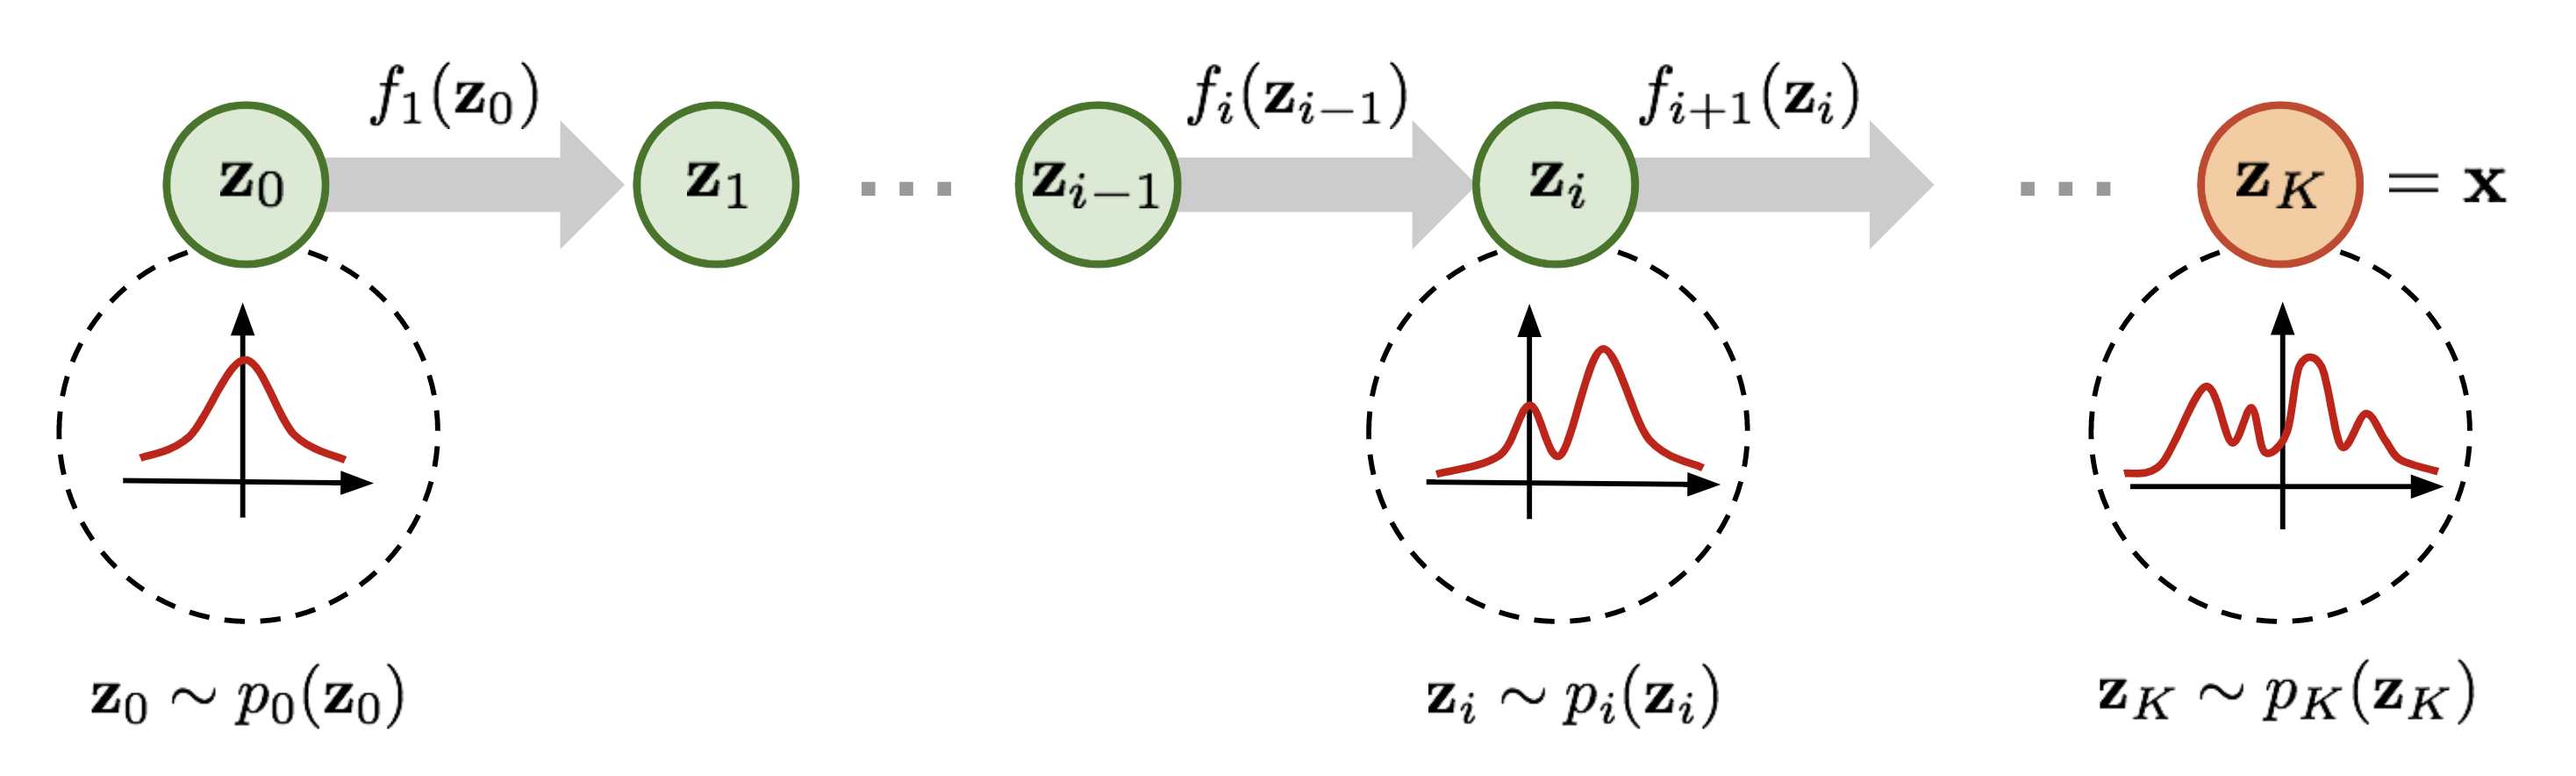
\includegraphics[scale=0.15]{Picture/norm_flow.png}
    \caption{正则流图例}
    \label{Norm_flow}
\end{figure}
对于连续函数$f:\mathbb{R}^{d}\rightarrow \mathbb{R}^d$,其中$f$可逆,定义$f$逆映射$f^{-1}=g$,即$g\circ f(z)=z$。如果我们用该映射将具有密度函数$q(z)$的隐式随机变量$z$映射到$z^{\prime}=f(z)$,则$z'$有如下密度函数
\begin{equation}
    q(z^{\prime}) = q(z)|\operatorname{det}\frac{\partial f^{-1}}{\partial z^{\prime}}|= q(z)|\operatorname{det}\frac{\partial f}{\partial z}|^{-1},
    \label{chain rule}
\end{equation}
其中最后一个等式可以利用链式法则来进行推广(如果有多个函数复合的情况下),我们可以复合多个函数并且循环利用式(\ref{chain rule})。对于有$K$个映射作用下得到的随机变量$z_{K}$(如图\ref{Norm_flow}中所示),由随机变量$z_0$连续变换$K$次得到的随机变量的密度函数$q_{K}(z)$具有性质
\begin{equation}
    \ln q_{K}(z_{K}) = \ln q_{0}(z_0)-\sum_{k=1}^{K}\ln |\operatorname{det}\frac{\partial f_k}{\partial z_{k-1}}|,
    \label{chain log likelihood}
\end{equation}
其中我们有
\begin{equation}
    z_{K}=f_{K}\circ \cdots f_1(z_0),
    \label{z_K definition}
\end{equation}
根据VAE模型的定义,我们的优化目标转换为如下目标:
\begin{equation}
    \ln p({x}) \geq \mathbb{E}_{q\left({z}^{(0)} \mid {x}\right)}\left[\ln p\left({x} \mid {z}^{(T)}\right)+\sum_{t=1}^T \ln \left|\operatorname{det} \frac{\partial {f}^{(t)}}{\partial {z}^{(t-1)}}\right|\right]-\mathrm{KL}\left(q\left({z}^{(0)} \mid {x}\right) \| p\left({z}^{(T)}\right)\right),
    \label{NF objective}
    \end{equation}
正则流可以用来逼近不同类型的VAE模型中的后验分布,只需要选取合适的转换函数$f^{(t)}$,不需要对编码器和解码器的结构进行修改,例如在\cite{papamakarios2021normalizing}中可以直接基于VAE模型的架构上去除隐空间变量的先验分布的假设,具有更强的泛化能力。在实际应用中,一般采取形式较为简单的可逆正则流(对每个元素进行运算而减少矩阵乘法的操作,从而不需要储存矩阵的逆提升计算速率)。以下列举代表性正则流例子。
\subsection{线性时间转换正则流模型(Invertible Linear-time Transformation)}
我们考虑如下形式的可逆变换
\begin{equation}
    f(z) = z+ u\cdot h(w^{\top } w + b),
    \label{family form}
\end{equation}
其中我们定义参数集$\lambda = \{w\in \mathbb{R}^{D}, u\in \mathbb{R}^D,b\in \mathbb{R}\}$ 为可以调节的参数,$h(\cdot)$为一个光滑非线性函数有导数$h'(\cdot)$,该映射对矩阵每一个元素进行相同的映射,为一个elementwise function。对于此类映射我们可以在$O(D)$复杂度时间内计算出对数雅可比项,计算如下
\begin{align}
    \psi(z) &= h'(w^{\top}z+b)w,\\
    |\operatorname{det}\frac{\partial f}{\partial z}| &= |\operatorname{det}(I+u\cdot \psi(z)^{\top})|=|1+u^{\top}\psi(z)|,
\end{align}
根据式(\ref{chain log likelihood})可以得到最终随机变量的似然函数以及根据在式(\ref{family form})中定义的正则流转换函数的形式可以得到在该族转换函数下的似然函数取值形式为
\begin{align}
     z_{K} &=f_{K}\circ \cdots f_1(z_0), \\
     \ln q_{K}(z_{K})&= \ln q_0(z)-\sum_{k=1}^{K}\ln |1+u_{k}^{\top}\psi_{k}(z_{k-1})|.
\end{align}
\subsection{扩散模型}
扩散概率模型在图像生成领域已经被证明是有效的生成模型,但是其缺点在于缺乏低维的有效隐藏变量$z$。然而,VAE模型通常具有低维有效的隐藏变量,可以通过结合两者来更加有效地
获得对高维数据分布的逼近。
和VAE模型一样,扩散模型的目的也是希望能够学习得到目标高维样本的分布性质。 在\cite{diffusion}中详细讨论了扩散模型的性质并且介绍了扩散模型的特殊情况,即DDPM模型用来对实际应用中的高维数据进行处理。以下部分中,我们首先将对扩散模型的数学原理进行回顾。基于随机微分方程的背景,假设有一个如下的随机微分方程
\begin{equation}
    dz = f(t)\cdot z \rm{dt}+g(t)\rm{dw}.
    \label{SDE 1}
\end{equation}
其中$\{z_t\}_{t=0}^{t=1}$为一个正向的连续变化的扩散过程,其中$z_0$为初始的随机变量,在此处我们将其作为想要研究的为止分布,而$z_t$则为在$t$时刻扩散得到的随机变量。其中, $f: \mathbb{R}\rightarrow \mathbb{R}$与
 $g: \mathbb{R}\rightarrow \mathbb{R}$为一维函数,$w$为标准布朗运动。可以通过设计$f$和$g$使得$z_1$服从标准正态分布,即$z_1\sim \mathcal{N}(z_1;0,I)$。而在实际对该连续变化过程进行采样的时候,通常会使用Euler法,即将$[0,1]$区间分成$T$个子区间$[i/T,(i+1)/T], i =0,1,\cdots, (T-1)$, 仅关注每一个子区间端点处随机变量的分布,即为$z_{i/T},i=0,1,\cdots,T$。在\cite{diffusion}中已经证明在式(\ref{SDE 1})中的随机微分方程可以通过一个生成式模型从尾端进行反转。在该文章中,在保证$z_1$服从标准正态分布的前提假设下,可以先对$z_1\sim \mathcal{N}(z_1;0,I)$进行取样,其次对逆向随机微分方程 $dz = \left[f(t)\cdot z -g(t)^2 \nabla_z \log q_t(z)\right] \rm{dt} + g(t)d \Tilde{w}$进行求解。其中$\Tilde{w}$为逆向标准布朗运动。在该逆向随机微分方程中,需要知道$\nabla_z \log q_t(z)$,即为在$t$时刻随机变量的正向传播下的边缘分布的打分函数(score function)。
 在\cite{diffusion}中训练逆向传播过程的参数只需要最小化如下量用来匹配打分函数
\begin{equation}
    \min _{{\theta}} \mathbb{E}_{t \sim \mathcal{U}[0,1]}\left[\lambda(t) \mathbb{E}_{q\left({z}_0\right)} \mathbb{E}_{q\left({z}_t \mid {z}_0\right)}\left[|| \nabla_{{z}_t} \log q\left({z}_t\right)-\nabla_{{z}_t} \log p_{{\theta}}\left({z}_t\right) \|_2^2\right]\right],
    \label{score objective 1}
\end{equation}
在此处我们还需要定义权重函数$\lambda(t)$。其中$q(z_0)$为目标样本的分布函数以及$q(z_t|z_0)$是扩散核,通过选取适当的$f(t)$和$g(t)$可以使得$q(z_t|z_0)$有解析表达式。在一般设定下由于不能保证有解析表达式,在\cite{diffusion}中将式(\ref{score objective 1})转换为优化如下目标
\begin{equation}
    \min _{{\theta}} \mathbb{E}_{t \sim \mathcal{U}[0,1]}\left[\lambda(t) \mathbb{E}_{q\left({z}_0\right)} \mathbb{E}_{q\left({z}_t \mid {z}_0\right)}\left[|| \nabla_{{z}_t} \log q\left({z}_t \mid {z}_0\right)-\left.\nabla_{{z}_t} \log p_{{\theta}}\left({z}_t\right)\right|_2 ^2\right]\right]+C,
    \label{score objective 2}
\end{equation}
其中$C=\mathbb{E}_{t \sim \mathcal{U}[0,1]}\left[\lambda(t) \mathbb{E}_{q\left({z}_0\right)} \mathbb{E}_{q\left({z}_t \mid {z}_0\right)}\left[\left\|\nabla_{{z}_t} \log q\left({z}_t\right)\right\|_2^2-\left\|\nabla_{{z}_t} \log q\left({z}_t \mid {z}_0\right)\right\|_2^2\right]\right]$,在
\cite{vincent}中说明了$C$的取值不取决于$\theta$,因此由式(\ref{score objective 2})和式(\ref{score objective 1})优化得到的参数$\theta$是等价的。为了计算上的便捷,通常会取$\lambda(t) = g(t)^2/2$, 其中在\cite{song_2}中说明了如果以如上方式选取权重函数$\lambda(t)$则可以使得在KL-散度意义下的目标分布和逆向SDE生成的分布的距离可以以式(\ref{score objective 1})作为上界,即
\begin{equation}
\operatorname{KL}\left(q\left({z}_0\right) \| p_{{\theta}}\left({z}_0\right)\right) \leq \mathbb{E}_{t \sim \mathcal{U}[0,1]}\left[\frac{g(t)^2}{2} \mathbb{E}_{q\left({z}_0\right)} \mathbb{E}_{q\left({z}_t \mid {z}_0\right)}\left[\left\|\nabla_{{z}_t} \log q\left({z}_t\right)-\nabla_{{z}_t} \log p_{{\theta}}\left({z}_t\right)\right\|_2^2\right]\right].
    \label{KL upper bound 1}
\end{equation}
在实际优化模型中,只需要对式(\ref{score objective 2})进行最小化即可,在得到相应模型参数$\theta$后对逆向随机微分方程进行求解可以得到对目标分布的逼近。由于扩散模型只需要保证末端的随机变量$z_1$服从正态分布,因此可以选取不同的$f(t)$,$g(t)$函数来生成目标分布。在接下来的部分中将着重分析一类特殊的扩散模型:DDPM模型。(Denoising Diffusion Probabilistic Models)
\subsection{降噪扩散概率模型(DDPM)}
在本部分将重新引入新的符号,这里我们定义$x_i= z_{i/T},i=0,1,\cdots,T$。
扩散模型为隐式变量模型满足如下形式$p_{\theta}(x_0) = \int p_{\theta}(x_{0:T}) dx_{1:T}$。其中$x_0=z_0\sim q(z_0)$为样本中的原始分布,$x_1,\cdots, x_{T}$ 为和$x_0$相同维数的隐式变量。 $x_T$对应一般扩散模型中的$z_1$,满足服从标准正态分布。由于$x_{0:T}$分别对应在$[0,1]$区间中的通过Euler法得到格点上的随机变量,由于此处可以假设$T$足够大,因此每一个相邻的条件概率分布$q(x_{i+1}|x_i)$都服从正态分布(利用布朗运动的性质)。\par 
首先开始定义正向过程,在正向过程中,扩散模型采用一步步向样本增加白噪声的方式,使得最终获得的随机变量$x_T$的分布趋近于正态分布。我们在此处通过选取参数$\beta_1, \cdots, \beta_{T}$ 的方式来选取每次增加噪声的大小。扩散模型的目的在于先用正向过程从$x_0$过渡到$x_T$使得其分布趋近于正态分布,再利用参数化得到的逆向过程来生成对初始样本分布的逼近。仿照逆向过程联合分布函数,正向联合分布函数的形式可以写为如下的形式:($\beta_t$用来定义相邻的条件概率分布的参数)
\begin{align}
    q\left(x_{1: T} \mid x_0\right)&=\prod_{t=1}^T q\left(x_t \mid x_{t-1}\right),\\
        q\left(x_t \mid x_{t-1}\right)&=\mathcal{N}\left(\sqrt{1-\beta_t} x_{t-1}, \beta_t I\right),
        \end{align}
        \begin{equation}
            q\left(x_t \mid x_0\right)=\mathcal{N}\left(\sqrt{\bar{\alpha}_t} x_0,\left(1-\overline{\alpha_t}\right) I\right) \text { 其中 } \alpha_t=\left(1-\beta_t\right) \text { 以及 } \bar{\alpha}_t=\prod_t \alpha_t,
            \label{posterior of xt}
            \end{equation}
    正向传播的后验分布同样可以被给出:
    \begin{equation}
        q\left(x_{t-1} \mid x_t, x_0\right)=\mathcal{N}\left(\tilde{\mu}_t\left(x_t, x_0\right), \tilde{\beta}_t\right),
        \label{posterior xt 2}
        \end{equation}
        \begin{equation}
            \text {     其中 } \tilde{\mu}_t\left(x_t, x_0\right)=\frac{\sqrt{\bar{\alpha}_{t-1}} \beta_t}{1-\bar{\alpha}_t} x_0+\frac{\sqrt{\alpha_t}\left(1-\bar{\alpha}_{t-1}\right)}{1-\bar{\alpha}_t} x_t,
            \end{equation}
            \begin{equation}
                \text { 以及 } \quad \tilde{\beta}_t=\frac{1-\bar{\alpha}_{t-1}}{1-\bar{\alpha}_t} \beta_t,
                \end{equation}
该正向过程实际上对应的随机微分方程即为
\begin{equation}
    dz = -\frac{g(t)^2}{2}\cdot  z dt + g(t)dw,
\end{equation}
$x_{0:T}$的联合分布$p_{\theta}(x_{0:T})$被称为逆向过程,并且它被定义为一个Markov过程,该过程的转移分布可以从末端$p(x_T)= \mathcal{N}(x_T;0,I) $开始。由此可以写出逆向过程的联合分布函数的表达式
\begin{equation}
    p_{\theta}(x_{0:T}) := p(x_T)\prod_{t=1}^{T}p_{\theta}(x_{t-1}|x_t), p_{\theta}(x_{t-1}|x_t) :=\mathcal{N}(x_{t-1};\mu_{\theta}(x_t,t),\Sigma_{\theta}(x_t,t)).  
\end{equation}

以上为正向Markov过程所满足的条件概率分布性质,在随机优化问题中为了优化参数需要对逆向传播过程进行建模。
逆向传播过程同样可以被参数化,此处使用高斯转移分布来进行此一阶Markov逆向传播过程,满足如下表达式:
\begin{align}
    p\left(x_{0: T}\right)&=p\left(x_T\right) \prod_{t=1}^T p_\theta\left(x_{t-1} \mid x_t\right),\\
        p_\theta\left(x_{t-1} \mid x_t\right)&=\mathcal{N}\left(\mu_\theta\left(x_t, t\right), \Sigma_\theta\left(x_t, t\right)\right).
        \end{align}
        \begin{figure}[H]
            \centering
            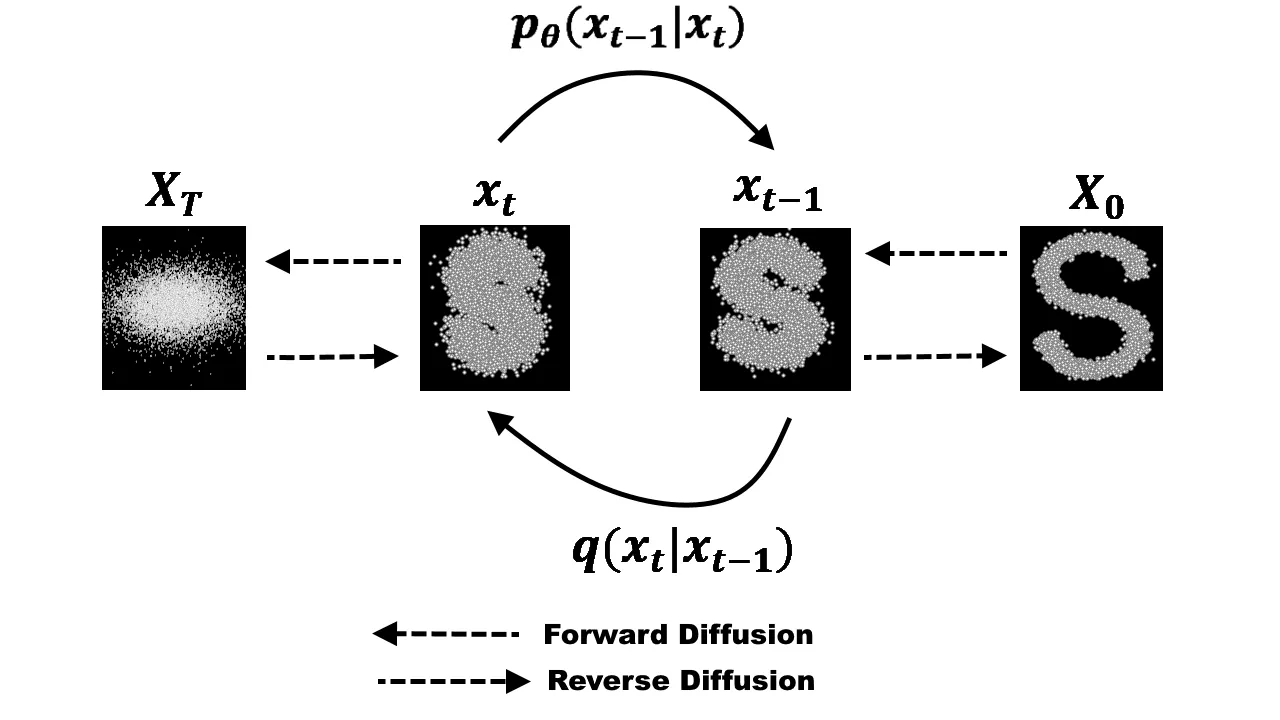
\includegraphics[scale = 0.2]{Picture/Diffusion.png}
            \caption{扩散模型图例}
            \label{Diffusion}
        \end{figure}
选取足够大的$T$值与合适的递减序列$\{\beta_t\}_{t\geq 1}$, 条件概率分布$q(x_{T}|x_0)$可以足够接近标准高斯分布。
整个概率系统可以通过变分推断来进行端到端的训练,从而优化参数。
在该模型下,同样采用极大似然估计的方式来进行参数优化,此处采用最大化对数似然函数的相反数的上界来进行优化,即
\begin{equation}
    \mathbb{E}\left[-\log p_\theta\left({x}_0\right)\right] \leq \mathbb{E}_q\left[-\log \frac{p_\theta\left({x}_{0: T}\right)}{q\left({x}_{1: T} \mid {x}_0\right)}\right]=\mathbb{E}_q\left[-\log p\left({x}_T\right)-\sum_{t \geq 1} \log \frac{p_\theta\left({x}_{t-1} \mid {x}_t\right)}{q\left({x}_t \mid {x}_{t-1}\right)}\right]=: L,
    \label{DDPM objective 1}
\end{equation}
从随机优化方法的角度去考虑,可以将式(\ref{DDPM objective 1})重新写为
\begin{equation}
\mathbb{E}_q[\underbrace{\mathcal{D}_{K L}\left(q\left(x_T \mid x_0\right) \| p\left(x_T\right)\right)}_{L_T}+\sum_{t>1} \underbrace{\mathcal{D}_{K L}\left(q\left(x_{t-1} \mid x_t, x_0\right) \| p_\theta\left(x_{t-1} \mid x_t\right)\right)}_{L_{t-1}}-\underbrace{\log p_\theta\left(x_0 \mid x_1\right)}_{L_0}].
    \end{equation}
以上为DDPM的数学原理,以下将具体讨论DDPM在实际优化过程中的参数设计与模型细节。以上已经将$L$分解成$L_T,L_{t-1},L_0$三大部分,由于后验分布$q$没有任何参数,因此$L_T$可以直接忽略(和$\theta$取值近似无关)。
在\cite{DDPM}中直接假设$\Sigma_{\theta}(x_t,t)=\sigma_t^2 I$,方便简化计算过程(避免矩阵求逆运算操作)。其次,为了表示$\mu_{\theta}(x_t,t)$,由于$p_{\theta}(x_{t-1}|x_t):= \mathcal{N}(x_{t-1};\mu_{\theta}(x_t,t),\sigma_t^2I)$,我们可以将$L_{t-1}$写为
\begin{equation}
    L_{t-1}=\mathbb{E}_q\left[\frac{1}{2 \sigma_t^2}\left\|\tilde{{\mu}}_t\left({x}_t, {x}_0\right)-{\mu}_\theta\left({x}_t, t\right)\right\|^2\right]+C,
    \label{Lt representation}
\end{equation}
其中$C$为一个和$\theta$无关的常数,在优化过程中可以被忽略。利用式(\ref{posterior of xt})可以进一步简化式(\ref{Lt representation}) 将$x_t$表示为${x}_t\left({x}_0, {\epsilon}\right)=\sqrt{\bar{\alpha}_t} {x}_0+\sqrt{1-\bar{\alpha}_t} {\epsilon} \text { for } {\epsilon} \sim \mathcal{N}({0}, {I}) $, 以及利用式(\ref{posterior xt 2})可以得到
\begin{align}
    L_{t-1}-C&=\mathbb{E}_{{x}_0, {\epsilon}}\left[\frac{1}{2 \sigma_t^2}\left\|\tilde{{\mu}}_t\left({x}_t\left({x}_0, {\epsilon}\right), \frac{1}{\sqrt{\bar{\alpha}_t}}\left({x}_t\left({x}_0, {\epsilon}\right)-\sqrt{1-\bar{\alpha}_t} {\epsilon}\right)\right)-{\mu}_\theta\left({x}_t\left({x}_0, {\epsilon}\right), t\right)\right\|^2\right]\\
&=\mathbb{E}_{{x}_0, {\epsilon}}\left[\frac{1}{2 \sigma_t^2}\left\|\frac{1}{\sqrt{\alpha_t}}\left({x}_t\left({x}_0, {\epsilon}\right)-\frac{\beta_t}{\sqrt{1-\bar{\alpha}_t}} {\epsilon}\right)-{\mu}_\theta\left({x}_t\left({x}_0, {\epsilon}\right), t\right)\right\|^2\right].
\end{align}
\subsection{去噪扩散隐式模型(DDIM)}
在DDPM的基础上,针对原模型所存在的缺陷,提出了DDIM,即去噪扩散隐式模型。在\cite{DDIM}中,针对DDPM所存在的缺陷,即每次进行优化需要生成整条Markov链需要较大计算复杂度的缺陷,提出了DDIM,即通过非Markov过程生成整条链。通过对比DDIM和DDPM的训练效果,发现DDIM可以生成更高质量的图像。接下来详细阐述DDIM模型正向生成样本的过程。
在正向传播过程中,Markov链的似然函数可以被写成如下形式:
\begin{equation}
    q_\sigma\left({x}_{1: T} \mid {x}_0\right):=q_\sigma\left({x}_T \mid {x}_0\right) \prod_{t=2}^T q_\sigma\left({x}_{t-1} \mid {x}_t, {x}_0\right),
\end{equation}
其中我们还有 $q_\sigma\left({x}_T \mid {x}_0\right)=\mathcal{N}\left(\sqrt{\alpha_T} {x}_0,\left(1-\alpha_T\right) {I}\right)$ 以及对与所有的$t>1$,我们还有
\begin{equation}
    q_\sigma\left({x}_{t-1} \mid {x}_t, {x}_0\right)=\mathcal{N}\left(\sqrt{\alpha_{t-1}} {x}_0+\sqrt{1-\alpha_{t-1}-\sigma_t^2} \cdot \frac{{x}_t-\sqrt{\alpha_t} {x}_0}{\sqrt{1-\alpha_t}}, \sigma_t^2 {I}\right),
\end{equation}
以及对于每个$t$,可以选择合适的均值函数,使得$q_\sigma\left({x}_t \mid {x}_0\right)=\mathcal{N}\left(\sqrt{\alpha_t} {x}_0,\left(1-\alpha_t\right) {I}\right)$。
根据贝叶斯公式,我们可以得到实际的条件分布密度函数为
\begin{equation}
   q_\sigma\left({x}_t \mid {x}_{t-1}, {x}_0\right)=\frac{q_\sigma\left({x}_{t-1} \mid {x}_t, {x}_0\right) q_\sigma\left({x}_t \mid {x}_0\right)}{q_\sigma\left({x}_{t-1} \mid {x}_0\right)},
   \label{Bayes Formula 1}
\end{equation}
根据式(\ref{Bayes Formula 1})可以得到如上分布依然为高斯分布。在该正向生成过程中,该链已经不满足Markov性质了。每次通过${x}_t,{x}_0$生成${x}_{t+1}$。接下来阐述反向传播链条的具体表达形式。首先,基于${x}_t$可以得到对于${x}_0$的一个估计,其次再利用两者的结合去预测${x}_{t-1}$。对于某个${x}_0\sim q({x}_0)$以及$\epsilon_t \sim \mathcal{N}(0,I)$,函数$\epsilon_{\theta}^{(t)}({x}_t)$旨在通过${x}_t$去预测$\epsilon_t$。通过函数$f^{(t)}_{\theta}$来进行对${x}_0$的预测。
\begin{equation}
f_\theta^{(t)}\left({x}_t\right):=\left({x}_t-\sqrt{1-\alpha_t} \cdot \epsilon_\theta^{(t)}\left({x}_t\right)\right) / \sqrt{\alpha_t}.
\end{equation}
如下可以定义反向传播过程,
\begin{equation}
 p_\theta^{(t)}\left({x}_{t-1} \mid {x}_t\right)= \begin{cases}\mathcal{N}\left(f_\theta^{(1)}\left({x}_1\right), \sigma_1^2 {I}\right) & \text { if } t=1 \\ q_\sigma\left({x}_{t-1} \mid {x}_t, f_\theta^{(t)}\left({x}_t\right)\right) & \text { 其余情形 }\end{cases}   
\end{equation}
通过变分推断的技术,可以计算得到ELBO的值,最后可以通过优化如下目标来得到参数$\theta$
\begin{align} & J_\sigma\left(\epsilon_\theta\right):=\mathbb{E}_{{x}_{0: T} \sim q_\sigma\left({x}_{0: T}\right)}\left[\log q_\sigma\left({x}_{1: T} \mid {x}_0\right)-\log p_\theta\left({x}_{0: T}\right)\right] \\ = & \mathbb{E}_{{x}_{0: T} \sim q_\sigma\left({x}_{0: T}\right)}\left[\log q_\sigma\left({x}_T \mid {x}_0\right)+\sum_{t=2}^T \log q_\sigma\left({x}_{t-1} \mid {x}_t, {x}_0\right)-\sum_{t=1}^T \log p_\theta^{(t)}\left({x}_{t-1} \mid {x}_t\right)-\log p_\theta\left({x}_T\right)\right],\end{align}
在实际优化中,不需要每次生成T个样本,可以只选取部分样本根据条件概率分布进行生成再进行优化。
\section{条件生成模型}
在实际应用中的诸多下游任务通常为条件生成图像的任务,例如图像去模糊化,图像修复,超分辨率图像生成等任务。 在数学上可以定义为,已知给定的图像$y\in \mathbb{R}^n$, 以及目标数据集$\mathcal{D}$, 目标为找到$\mathcal{D}$中的一个子分布$\mathcal{D}^{\prime}\subseteq \mathcal{D}$ 使得 $\mathcal{D}^{\prime}$为在极大似然意义下$y$在前向加噪算子$H$的原像。 相比于在无条件生成下的情形,条件生成需要同时结合先验条件$y$的信息以及目标生成图像数据集$\mathcal{D}$的信息。 通常我们可以表述为,
\begin{equation}
    y = Hx +b ,  x\in \mathcal{D},\label{condition model}
\end{equation}
其中$b$可以取为某常数或者随机高斯噪声,目标为在给定$y$的情形下找到所有满足式(\ref{condition model})的$x$的分布,即可以采样获得所有满足条件的$x$。      


利用\cite{score_based_SDE,song_2}中利用score function来逆向采样方法,此时的score function拥有$s_{\theta}(t,z_t,y)$的形式。但是如果仅仅利用该方法去重新训练一个模型获得打分函数,不仅在计算资源上较为昂贵,同时对于不同的向前加噪算子$H$就需要训练不同的模型,在泛化能力上也较为局限。在条件生成下,目标score function变为
\begin{equation}
    s(t,z_t\mid y) = \nabla_{z_t}\log\left(q(z_t\mid y)\right)= \nabla_{z_t}\log(q(z_t)+\nabla_{z_t}\log \left(q(y\mid z_t)\right).
    \label{Bayes transformation}
\end{equation}
在使用预训练集的情况下,我们只需要得到$\nabla_{z_t}\log(q(y\mid z_t))$的值即可,通常而言条件生成有以下几种解决思路。

\section{分类器辅助 }
\label{classifier guidance}
分类器辅助(Classifier Guidance)用于辅助使得生成的图像属于目标数据集,即此时我们使用如下逼近方法:
\begin{equation}
    \nabla_{{z}_t} \log q\left({z}_t \mid y\right)\approx \nabla_{{z}_t} \log q\left({z}_t\right)+\lambda \nabla_{{z}_t} \log q\left(y \mid {z}_t\right),
\end{equation}
其中$\lambda$为一个可调节的超参数用来控制权重, 该方法的缺点在于需要预训练集对带噪声的输入具有一定的鲁棒性,而该性质对常见数据集的预训练集通常不适用。 


\section{无分类器辅助}
相比于在\ref{classifier guidance}中提到的分类器辅助的方法,我们可以引入无分类器辅助的方法,此时我们采用如下逼近方法
\begin{equation}
    \nabla_{{z}_t} \log q\left({z}_t \mid y\right)\approx (1-\lambda)\nabla_{{z}_t} \log q\left({z}_t\right)+\lambda \nabla_{{z}_t} \log q\left( {z}_t \mid y \right),
\end{equation}
因此我们可以得到两个score function分别为在无条件生成下的score function $\nabla_{{z}_t} \log q\left({z}_t\right)$ 和条件生成意义下的score function$\nabla_{{z}_t} \log q\left( {z}_t \mid y \right)$。当我们取$\lambda=0$ 时退化成为无条件生成的模式, 取$\lambda=1$的时候则和标准的条件生成问题相同。 最为有趣的情况为当取$\lambda=1$的时候,此时在$\nabla_{{z}_t} \log q\left({z}_t\right)$前面的系数$<0$,更大程度的增大了和先验信息$y$相匹配的可能性。 但是该方法的主要问题在于,需要同时训练两个模型,在计算资源上同样较为昂贵,实现成本较大。 

\section{投影方法}
\label{projection based}
对于解决逆向生成问题,本质上需要从原像$H^{-1}(y)$中寻找一个在原数据集$\mathcal{D}$上的一个投影,因此在本部分旨在寻找投影方法使得可以将原像投影到数据集空间(通常我们可以假设某一个数据集为在图像所处高维空间中的一个低维嵌入,因此相当于只需要找原像集合在该子空间的投影即可)。具体而言,例如在从低分辨率图像还原的下游任务中,投影法旨在从低分辨率(LR)图像中提取固有结构或纹理,以在每一步补充生成的图像并确保数据一致性。一个关于修补任务中基于投影方法的示例是\cite{PnP}。在图像修复任务中中,扩散过程被选择性地应用于需要修补的特定区域,而保留图像的其余部分不变。受到此概念的启发,\cite{red_diff}应用了类似的技术。 
在\cite{MCG}中利用如下方法来进行迭代更新
\begin{align} & \hat{{z}}_{t-1}=\mathrm{f}\left({z}_t, t\right)+\mathrm{g}\left({z}_t, t\right) \cdot \varepsilon_t, \\ & {z}_{t-1}=({I}-{P}) \cdot \hat{{z}}_{t-1}+\hat{{y}}, \quad \hat{{y}} \sim q\left({z}_t \mid {z}_0=y\right),\end{align}

其中$f$, $g$的形式取决于具体的扩散模型选取,而$P$算子即为具体的低分辨率算子。

\section{分解方法}
同样以超分辨率还原下游任务举例,此时式(\ref{condition model})在该情形下可以表示为
\begin{equation}
y  = A x +b,
    \label{super resolution example }
\end{equation}
$A$为低分辨率算子为线性算子, $b$为外界干扰噪声。 由于线性算子的形式较为简洁我们同样可以定义线性空间下的Moore-Penrose逆 $A^{\dagger}$,即满足 
\begin{equation}
   A^{\dagger} A A^{\dagger}= A^{\dagger} , AA^{\dagger}A = A.  
   \label{definition of moore-penrose inverse}
\end{equation}
则在不考虑原像分布的情况下,原像取如下形式
\begin{equation}
    \hat{x} = A^{\dagger} y + (I - A A^{\dagger})\Bar{x}. \label{decompostion null space}
\end{equation}
在\cite{ddnm}中就运用式(\ref{decompostion null space}),从而只需要对$\Bar{x}$进行采样即可,第一项已经用到了所有先验信息。 

\section{后验估计}
根据式(\ref{Bayes transformation}),在使用预训练集下,只需要通过估计后验分布的打分函数即可对条件生成问题进行采样。在\cite{Inverse,MCG}中主要针对后验估计来进行算法设计。 
考虑在加噪模型式(\ref{super resolution example })下,结合式(\ref{Bayes transformation},我们采取如下逼近方式
\begin{align} \nabla_{\mathbf{z}_t} \log p_t\left(\mathbf{x} \mid \mathbf{z}_t\right) & \approx \nabla_{\mathbf{z}_t} \log p\left(\mathbf{x} \mid \hat{\mathbf{z}}_0\left(\mathbf{z}_t\right)\right) \\ & \approx-\frac{1}{\sigma^2} \nabla_{\mathbf{z}_t}\left\|\mathbf{x}-A\left(\hat{\mathbf{z}}_0\left(\mathbf{z}_t\right)\right)\right\|_2^2.\end{align}
其中我们假设噪声服从无偏正态分布,即$n\sim \mathcal{N}\left(0,\sigma^2 I\right)$ ,$\hat{z}_0(z_t) = \mathbb{E}\left[z_0\mid z_t\right]$因此可以表示为关于$z_t$的函数$\hat{z}_0(z_t)$。利用对条件分布意义下的score function的逼近可以以此进行采样估计。 

\section{小结}
在本文的前两部分中,我们分别探讨了非条件生成与条件生成中涉及的数学模型和实现原理。

在非条件生成部分,主要讨论了变分自编码器(VAE)模型和扩散(Diffusion)模型。在VAE模型中,为了减轻隐变量需满足标准正态先验的假设,可以采用正则流技术来放宽这一条件,并通过链式法则进行随机优化。在扩散模型中,根据不同的采样方法,模型可以进一步扩展为深度确定性政策梯度(DDPM)等。基于DDPM,通过优化采样技术,衍生出如DDIM等新型生成模型来解决生成步骤较长的问题,并显著提高了图像生成的效率。在最新的研究中,例如Stable Diffusion模型,通过结合VAE模型将高维图像压缩至低维隐空间的特性,以及扩散模型的优势,实现了更高效的图像生成。但由于计算资源的限制,本文不对这一领域的应用进行详尽讨论。

在条件生成的部分,本文详细探讨了如何构建条件分布下的Score Function来进行有效的图像生成。具体来说,通过利用条件信息,可以指导生成过程以满足特定的需求或约束,从而产生具有目标特征的图像。

首先,我们考虑分类器辅助方法,该方法通过在训练阶段引入预训练的分类器来增强生成模型的条件约束能力。这种方式不仅可以确保生成的图像质量,还可以通过分类器的指导来调整生成过程,使生成的图像更加符合特定类别的特征。然而,这种方法对计算资源的依赖较大,需要较高的计算能力和存储空间。

接下来,无分类器辅助方法通过直接在Score Function中融入条件变量来实现条件生成。这种方法避免了依赖外部分类器,减少了模型复杂度,但同时对Score Function的设计和优化提出了更高的要求。通过精细调整条件变量的权重,可以在不牺牲生成质量的前提下,直接在模型内部控制生成过程的方向和特性。

此外,使用投影或分解技术也是实现条件生成的一种有效手段。通过这些技术,可以将高维的数据投影到较低维的特定子空间,这个子空间能够捕捉到与条件相关的关键特征。这种方法有助于改善生成模型的训练效率和样本的多样性,同时保持生成图像的相关性和准确性。

最后,后验估计技术在条件生成中也发挥着重要作用。通过对后验分布的Score Function进行精确估计,可以更好地理解和控制生成过程中的随机性和不确定性,从而提高生成模型的稳定性和可靠性。

综上所述,通过这些方法的结合使用,可以在保证生成图像质量和相关性的同时,有效地实现条件生成,为后续的图像修复任务提供了坚实的理论和技术基础。



% \subsection{VAE模型和扩散模型的结合:隐式扩散模型}
% 结合扩散模型的优点,可以去除在VAE模型中隐式变量$z$的先验分布为标准正态分布的假设。在得到隐式变量$z$后,先通过一个扩散模型学习到$p_{\theta}(z_0)$用来逼近$z_0$的真实分布,然后再通过解码器生成$x$的分布。接下来我们对该混合模型的原理进行具体回顾,在\cite{VAE_diffusion}中对该方法进行了详细的阐述。对于传统VAE模型,隐含假设为隐式变量$z$的先验分布为标准正态分布,然而该假设对于现实生活中许多具有离散分布的数据并不成立。因此需要通过扩散模型去学习到真实的隐式变量的分布,接下来详细说明该模型的执行流程。
% 在该模型下,我们依然只考虑如下形式的随机微分方程进行扩散
% \begin{equation}
%     dz = f(t)\cdot zdt + g(t)dW_t
%     \label{SDE form }
% \end{equation}
% 其中$\{W_t\}_{t\geq 0}$为标准布朗运动
% \begin{figure}[H]
%     \centering
%     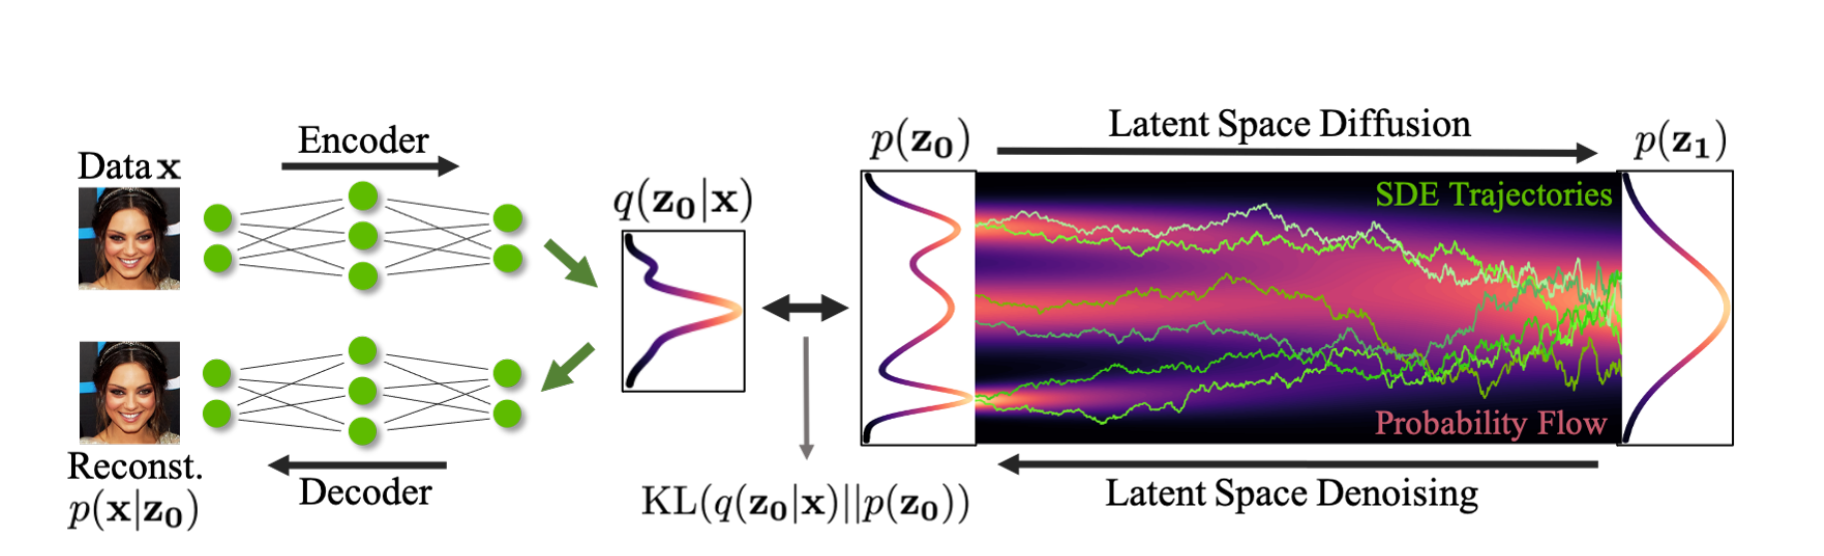
\includegraphics[scale = 0.5]{Picture/VAE_diffusion.png}
%     \caption{VAE模型和扩散模型的结合}
%     \label{fig_VAE_Diffusion}
% \end{figure}
% 在图\ref{fig_VAE_Diffusion}中,由三部分组成:编码器$q_{\phi}(z_0|x)$, 扩散模型$p_{\theta}(z_0)$和解码器$p_{\psi}(x|z_0)$。首先样本$x$利用编码器得到隐式变量$z_0$,再通过扩散模型通过$z_0$扩散到$z_1$使得$z_1$服从标准正态分布$z_1\sim \mathcal{N}(z_1;0,I)$。利用逆向微分方程可以从末端$z_1$开始取样通过解方程采样得到$z_0$的分布的近似$p_{\theta}(z_0)$。最后,通过解码器可以通过$p_{\psi}(x|z_0)$将隐式变量映射到原先的样本空间中。在该模型中,和VAE模型的处理方法相同,我们依然通过极大似然估计的方法去进行参数训练。我们在此处最小化对数似然函数相反数的下界(ELBO)来进行参数估计,
% \begin{align}
%  \mathcal{L}({x}, {\phi}, {\theta}, {\psi})&=\mathbb{E}_{q_{{\phi}}\left({z}_0 \mid {x}\right)}\left[-\log p_{{\psi}}\left({x} \mid {z}_0\right)\right]+\operatorname{KL}\left(q_{{\phi}}\left({z}_0 \mid {x}\right) \| p_{{\theta}}\left({z}_0\right)\right) \label{Loss decomposition 1}\\
% & =\underbrace{\mathbb{E}_{q_{{\phi}}\left({z}_0 \mid {x}\right)}\left[-\log p_{{\psi}}\left({x} \mid {z}_0\right)\right]}_{\text {reconstruction term }}+\underbrace{\mathbb{E}_{q_\phi\left({z}_0 \mid {x}\right)}\left[\log q_{{\phi}}\left({z}_0 \mid {x}\right)\right]}_{\text {negative encoder entropy }}+\underbrace{\mathbb{E}_{q_{{\phi}}\left({z}_0 \mid {x}\right)}\left[-\log p_{{\theta}}\left({z}_0\right)\right]}_{\text {cross entropy }} \label{loss decomposition 2}
% \end{align}
% 通过式(\ref{loss decomposition 2})可以将式(\ref{Loss decomposition 1})中的KL散度进行进一步分解。在式(\ref{loss decomposition 2})中的reconstruction term 和 encoder entropy term都可以通过VAE模型中所使用的重参数化技巧来进行估计优化,在优化中最困难的部分是对交叉熵部分进行估计求导。以下引用在\cite{VAE_diffusion}中得到的关于交叉熵的结论。
% \begin{theorem}
% 在随机微分方程式(\ref{SDE form })下,考虑两个初始分布$q(z_0)$和$p(z_0)$,都定义在$\mathbb{R}^{D}$上,假设$q(z_t)$ ,$p(z_t)$代表在SDE(\ref{SDE form })下在$t\in [0,1]$时刻扩散得到的随机变量的边缘分布。同时假设$\log(p(z_t))$和$\log(q(z_t))$均为光滑函数且在$z_t\to \infty$时增长速度不超过多项式量级增长。同时我们假设所选取的$f(t)$
% $g(t)$满足在$t=1$时刻满足$q(z_1)=p(z_1)$,则交叉熵满足以下等式
% \begin{align}
%     \operatorname{CE}\left(q\left({z}_0 \mid {x}\right) \| p\left({z}_0\right)\right) &=\mathbb{E}_{t \sim \mathcal{U}[0,1]}\left[\frac{g(t)^2}{2} \mathbb{E}_{q\left({z}_t, {z}_0 \mid {x}\right)}\left[\left\|\nabla_{{z}_t} \log q\left({z}_t \mid {z}_0\right)-\nabla_{{z}_t} \log p\left({z}_t\right)\right\|_2^2\right]\right] \nonumber\\
%     &+\frac{D}{2} \log \left(2 \pi e \sigma_0^2\right) \label{thm 1}
% \end{align}
%     其中$q(z_t,z_0|x) = q(z_t|z_0)q(z_0|x)$,以及条件概率分布$q(z_t|z_0)$为正态分布有如下形式$q(z_t|z_0)=\mathcal{N}(z_t;\mu_t(z_0),\sigma_t^2)$。其中$\mu_t$,$\sigma_t^2$由$f(t)$和$g(t)$以及初始时刻$t=0$处方差$\sigma_0^2$唯一确定。
% \end{theorem}
% 根据以上结论,在实际优化过程中需要对$t$时刻的随机变量$z_t$进行采样来进行随机梯度下降,然而根据该种采样得到的随机变量可能有较高的方差,在实际优化中需要采用一定的减小采样方差的方法。 在实际应用中通常会对VPSDE(Variance Preserving SDE)进行分析,即SDE形式为
% \begin{equation}
%     dz = -\frac{1}{2}\beta(t)zdt + \sqrt{\beta(t)}dW.
%     \label{VPSDE}
% \end{equation}
% 其中我们可以定义$\beta(t) = \beta_0+(\beta_1-\beta_0)t$,从而使得该函数取值始终在$[\beta_0,\beta_1]$内。(也可以更换该函数形式满足更加复杂的应用需求)
% 在\cite{Consistency}中对一致性模型的诸多性质进行了详细的阐述。\par 
% 在实际应用中,由于图像的维数相对较高,如果直接使用Diffusion Model进行训练(例如使用DDPM等模型)会带来较大的计算资源消耗,因此通常会先将图像通过编码器映射到隐空间中,通过Diffusion Model训练得到隐空间变量的真实分布,最后再通过解码器得到还原后的图像。该方法可以用于图像去噪,图像生成等下游任务。在\cite{High_synthesis}中详细阐述了使用VAE模型和Diffusion Model的结合在图像生成中的丰富应用。以及如果再充分使用Transformer模型,可以进一步实现文字转图像等丰富功能。

